\chapter{Background}
\label{chap:background}
\section{Docker}
Docker \cite{Docker} is a open-source project container engine. It provides an additional layer of abstraction and automation of operating-system-level virtualization in Linux. Docker has two parts, including Docker client and Docker daemon.

\begin{figure}[h]
\begin{center}
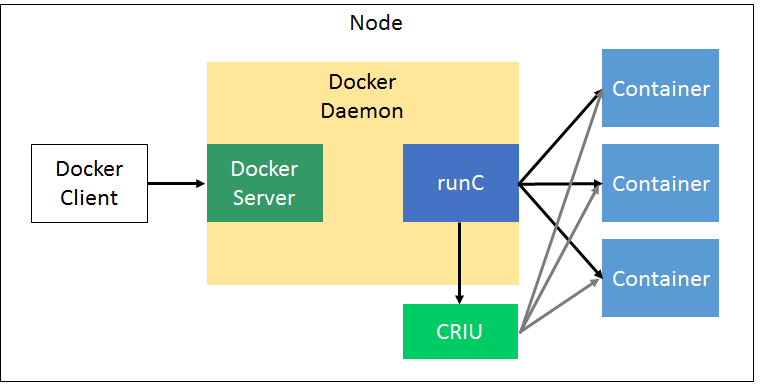
\includegraphics[width=10cm]{figure/single_node.png}
\end{center}
\caption{Single node Docker}
\end{figure}

\subsection{Docker client}
Docker is typical Client/Server architecture application. Docker client uses Docker command to send and receive requests to Docker Daemon. Also, Docker supports remote RESTful API to send and receive HTTP requests to Docker Daemon. In additional, it has been implemented by more than 10 programming languages.

\subsection{Docker daemon}
Docker daemon is a daemon that runs as system service. It has two the most importance features: 
\begin{itemize}
    \item Receive and handle Docker client's requests.
    \item Manage containers.
\end{itemize}
When docker daemon is running, it will run a server that receives requests from Docker clients or remote RESTful API. After receiving requests, server will pass the requests by router to find the handler to handle the requests.

\subsection{runc}
runc is a CLI tool for running containers according to the OCI specification. It doesn't need any dependency from the system, it can control Linux Kernel include namespace, cgroups, apparmor, netlink, capabilities, firewall, etc.
runc provides a standard interface to support the containers management. Docker can use runc to control the containers.

\section{Docker Swarm}
Docker Swarm is a native clustering for Docker. It gathers several docker engines together into  one virtual docker engine. Docker Swarm serves standard Docker API, so it can be connected by Dokku, Docker Machine, Docker Compose, Jenkins, DockerUI, Drone, etc. It also support Docker client of course.
In Docker Swarm, it has two components which are Swarm master and Swarm node. Swarm master is the manager which handles Docker client and RESTful API requests and manages multiple Docker nodes resources. Docker node is an agent which sends heartbeat to Discovery Service to ensure Docker daemon is alive in the cluster.
\\
\\
\\
\begin{figure}[h]
\begin{center}
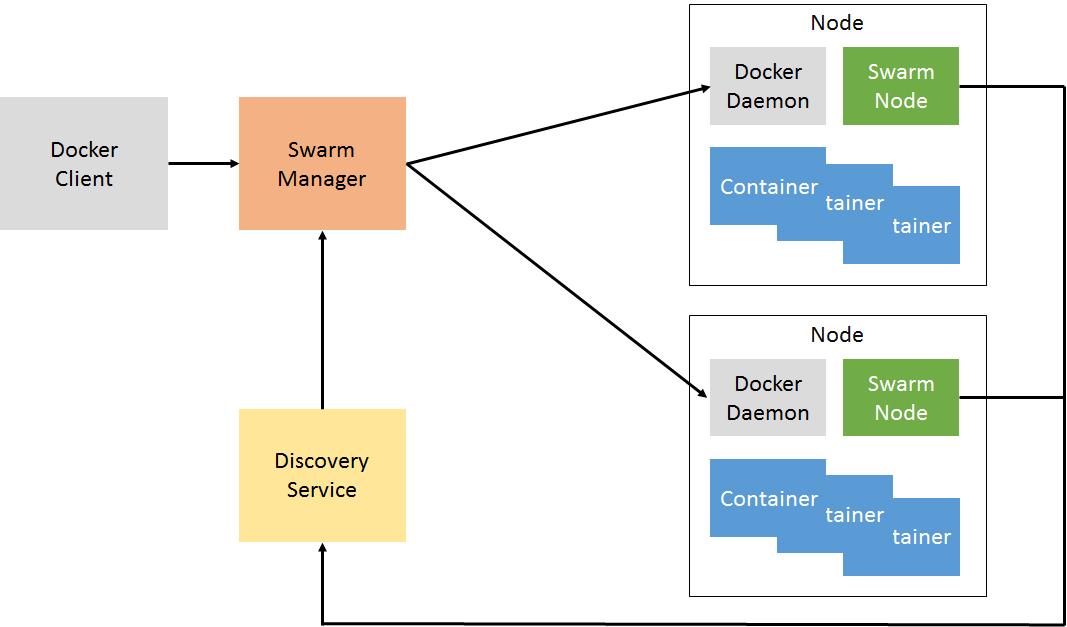
\includegraphics[width=15cm]{figure/swarm_docker.png}
\end{center}
\caption{Docker Swarm architecture}
\end{figure}

\subsection{Discovery services}
Docker Swarm provides multiple Discovery Services backends. They are used to discover nodes in the cluster. There are:
\begin{itemize}
    \item Using a distributed key/value store, like Consul, Etcd and Zookeeper.
    \item A static file or list of nodes.
    \item Docker Hub as a hosted discovery service
\end{itemize}
Otherwise, it also supports any modules which satisfy Discovery API interface.

\subsection{Scheduler}
Docker Swarm scheduler decides which nodes to use when creating and running a container. It has two steps. First, It follows user's filters to decide which nodes are conform. Second, It passes through strategies to select the best node in the cluster.

\subsubsection{Filter}
Filters are divided into two categories, node filters and container configuration filters. Node filters operate on characteristics of the Docker host or on the configuration of the Docker Daemon. Container configuration filters operate on characteristics of containers, or on the availability of images on a host.
The node filters are:
\begin{itemize}
    \item Constraint
    \item Container slots
    \item Health filter
\end{itemize}
The container configuration filters are:
\begin{itemize}
    \item Affinity
    \item Dependency
    \item Port filter
\end{itemize}

\subsubsection{Strategies}
The Docker Swarm scheduler features multiple strategies for ranking nodes. Swarm currently supports these values:
\begin{itemize}
    \item Spread
    \item Binpack
    \item Random
\end{itemize}
Spread and Binpack strategies compute rank according to a node’s available CPU, its RAM, and the number of containers it has. It selects a node at random. Under the Spread strategy, Swarm optimizes for the node with the least number of containers. The Binpack strategy causes Swarm to optimize for the node which is most packed. The Random strategy uses no computation, chooses nodes at random regardless of their available CPU or RAM.

\subsection{High availability}
In Docker Swarm, Swarm manager responses the cluster and manages the resources of multiple Docker nodes at scale. If Swarm master dies, we have to create a new one and deal with the interruption of service.
The High availability feature allows Docker Swarm has multiple Swarm manager instances. We can create a primary manager and multiple replica instances. Whenever we send requests to replica instances, it will be automatically proxied to the primary manager. In addition, if the primary manager fails, the others replica instances will lead a new primary manager.

\section{CRIU}
CRIU \cite{CRIU} (Checkpoint/Restore in Userspace) stands for Checkpoint and Restore in User Space, creates a complete snapshot of the state of a process, including things like memory contents, file descriptors, and even open tcp connections. It can be used for suspending and resuming processes, or live migrating them from one machine to another.

\ref{chap:background} and cite test \cite{Sohi:1995:MP:225830.224451, Hammond:1998:DSS:291069.291020, grinberg2009parallel}.